\documentclass[ mode = beamer, handout ]{hduthesis}

\usepackage[mono = false]{libertine}
\hduset
  {
    title      = Beamer Theme for Hangzhou Dianzi University
                 Based on \LaTeX3,
    subtitle   = hdu Undergraduate Thesis Proposal,
    author     = SAN Chi Nan (C668668E0),
    date       = {\today{} / Xiasha Campus},
    supervisor = Prof. YIP Tsz Ching,
    bibsource  = reference.bib,
  }

\begin{document}

\maketitle

\section{Research Methods}

\begin{frame}{Landau-Lifshitz-Gilbert Equation}
  \pause
  Landau-Lifshitz-Gilbert (LLG) equation describes the microkinetics of magnetization in ferromagnetic materials. It combines the Landau-Lifshitz (LL) equation and the Gilbert damping term $\alpha$, which is used to simulate and understand the micro-magnetic dynamics phenomena such as the motion of magnetic domain walls and magnetization reversal.
  \pause
  \begin{equation}
    \odv{\mathbf m}{t} = -\gamma \mathbf m \times \mathbf H_\text{eff} -
    \boxed{\alpha \mathbf m \times \odv{\mathbf m}{t}}
  \end{equation}
  \pause
  To process the term $\alpha \mathbf m \times \odv{\mathbf m}/{t}$,
  we left multiply the LLG equation by $\mathbf m$ and use the identity
  $\mathbf m \cdot \odv{\mathbf m}/{t} = 0$ to generate LL equation.
  \pause
  \begin{equation}
    \odv{\mathbf m}{t} = -\frac{\gamma}{1 + \alpha^2} \mathbf m \times \mathbf H - \frac{\gamma\alpha}{1 + \alpha^2} \mathbf m \times \mathbf m \times \mathbf H
  \end{equation}
  \pause
  \alert{The LLG equation is more convenient for numerical calculation, while the LL equation can introduce the dissipation term more physically.}
\end{frame}

\begin{frame}{Applications}
  \pause
  \begin{block}{Magnetic Memory}
    Magnetic memory is a type of non-volatile memory that uses magnetic fields to store data. It is a type of computer memory that does not require power to maintain the information stored in the memory.
  \end{block}
  \pause
  \begin{exampleblock}{Magnetic Logic}
    Magnetic logic is a type of logic gate that uses magnetic fields to perform logical operations. It is a promising technology for future computing systems.
  \end{exampleblock}
  \pause
  \begin{alertblock}{Magnetic Sensor}
    Magnetic sensors are devices that detect magnetic fields. They are used in a wide range of applications, including automotive, industrial, and consumer electronics.
  \end{alertblock}
  Lorem\cite{xu2023unified},
  Ipsum\cite{wang2023electrical},
  dummy\cite{haug2008quantum},
  text\cite{wang2024switching,jhuria2020spin, gilbert2004phenomenological, foros2005magnetization,
        chudnovskiy2008spin, foros2009noise, swiebodzinski2010spin,
        brataas2008scattering, brataas2011magnetization}
\end{frame}

\begin{frame}{The NEGF Method}
  \pause
  The Nonequilibrium Green Function (NEGF) method can be used to study the quantum transport properties of nanoscale devices, such as quantum dots, nanowires, and molecular junctions. The four important Green's functions in the NEGF method are
  \pause
  \begin{equation}
    \begin{cases*}
      G^r = -i\theta(t - t') \ab\big<\{a_i(t), a_j^\dagger(t)\}> & Retarded Green's function\\
      G^a = i\theta(t' - t) \ab\big<\{a_i(t), a_j^\dagger(t')\}> & Ahead Green's function\\
      G^< = i\ab\big<\{a_j^\dagger(t'), a_i(t)\}> & Lesser Green's function\\
      G^> = -i\ab\big<\{a_j^\dagger(t'), a_i(t)\}> & Greater Green's function
    \end{cases*}
  \end{equation}
  \pause
  And sometimes we need multiply anchors on the contour of time.
  \begin{center}
    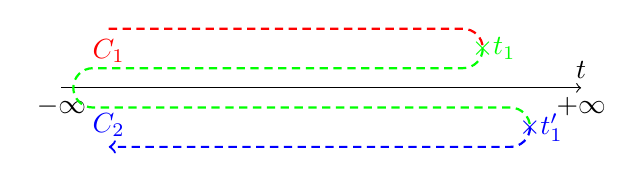
\begin{tikzpicture}
      \draw [->] (-3.6,0) -- (3,0) node [anchor=south] {$t$} node [anchor=north] {$+\infty$} node [at start,anchor=north] {$-\infty$};
      \draw [densely dashed, red,thick] (-3,0.75) -- (1.5,0.75) node [at start,anchor=north] {$C_1$} arc (90:0:0.25);
      \draw [densely dashed, green, thick] (1.75,0.5) arc (0:-90:0.25) node [at start] {$\times$} node [at start, anchor=west] {$t_1$} -- (-3.2,0.25) arc (90:270:0.25) -- (2.1,-0.25) arc (90:0:0.25);
      \draw [densely dashed, ->, blue, thick] (2.35,-0.5) arc (0:-90:0.25) node [at start] {$\times$} node [at start,anchor=west] {$t_1'$} -- (-3,-0.75) node [anchor=south] {$C_2$};
    \end{tikzpicture}
  \end{center}
\end{frame}

\printbibliography

\end{document}